\section{Method} \label{sec:method} 

In this section we will describe the method we have used to solve the Authorship
Verification problem presented. In general there are two methods of representing
each author. There is the instance based approach and the profile based
approach. In the instance based approach each author is represented by a set of
texts they have written while in the profile based approach they are represented
by the sum of the set of texts they have written. The instance based approach is
illustrated in Figure \ref{fig:instance_based} and the profile based approach is
illustrated in Figure \ref{fig:profile_based}.

\begin{figure}[htb]
    \centering
    \textbf{Instance Based Authorship Verification or Authorship Attribution}
    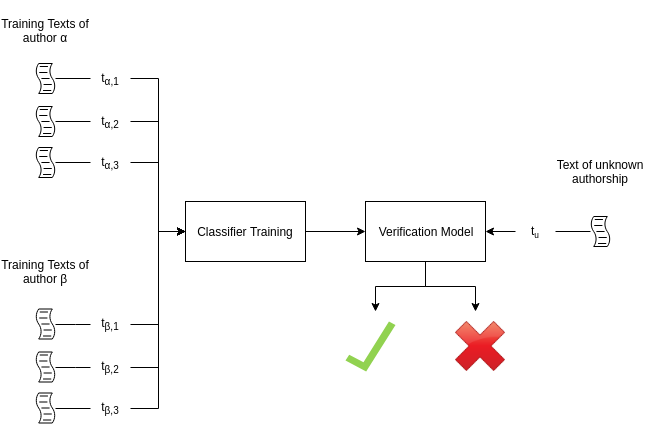
\includegraphics[scale=0.5]{./pictures/method/InstanceBased.png}

    \caption{Illustrate the typical instance based Authorship Verification or
    Authorship Attribution solution setup. Inspired by \cite{stamatos2009} a
    set of authors are given as input each with a set of texts. Some Machine
    Learning model is trained on the input texts and the model is used to
    predict an unknown text. }

    \label{fig:instance_based}
\end{figure}

\begin{figure}[htb]
    \centering
    \textbf{Profile Based Authorship Verification or Authorship Attribution}
    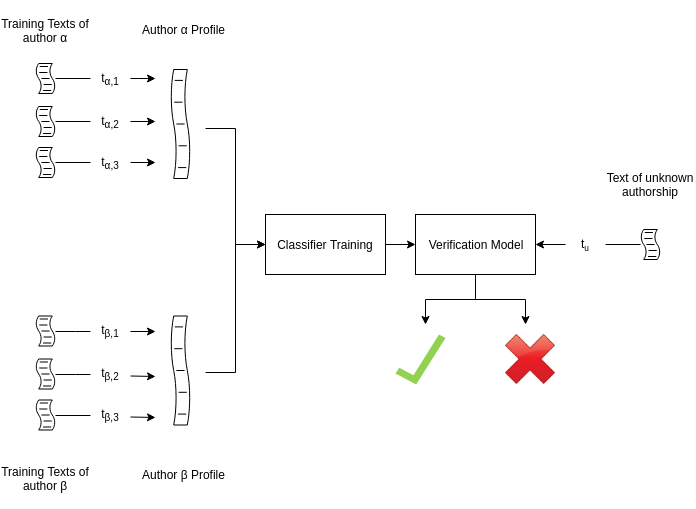
\includegraphics[scale=0.5]{./pictures/method/ProfileBased.png}

    \caption{Illustrate the typical profile based Authorship Verification or
    Authorship Attribution setup. Inspired by \cite{stamatos2009} the texts of
    each author are combined using some combination function such as an average
    or a concatenation. Those \textit{profiles} are then given to a Machine
    Learning model to train. The output is a model which is used to predict
    unknown texts. }

    \label{fig:profile_based}
\end{figure}

We will generally use the instance based approach. The reason we use an instance
based approach is that it allows us to use extra information from each single
text. For example writing style may change over time especially for secondary
school pupils that evolve very much in a short amount of time. Since we use an
instance based approach we are able to weight similarity to newer texts higher
than similarity to older texts.

There are also another split between methods that we consider. There are
generalizing and author specific models. In a generalizing model only a single
model is trained on data from multiple authors and are able to make predictions
about previously unseen authors. In the author specific model a separate model
has to be trained for each author and is not able to make predictions for
previously unseen authors. The generalizing model has several advantages, it
only has to be trained once and after that it can be used for everyone and
it can make use of big data since it can use data from several authors for
training. The author specific model has the advantage that it can better fit
to the specific quirks of a particular author since it is trained separately
for each author. The downside of the author specific approach is that a new
model has to be trained for each new author. We will focus on the generalizing
approach since it is easier to implement for MaCom as they only have to train a
model once.

As a unit of measuring the quality of our models, and how well they adhere to
95\% specificity constraint, we will also compute the number of \gls{TP}s,
\gls{TN}s, \gls{FP}s and \gls{FN}s, as was done in a project previously created
by us.\cite{US} In these problems we get,

\begin{itemize}
    \item a \gls{TP} whenever we answer \textit{True} and the texts are written
        by the same author,
    \item a \gls{TN} whenever we answer \textit{False} and the texts are
        \textbf{not} written by the same author,
    \item a \gls{FP} whenever we answer \textit{True} and the texts are
        \textbf{not} written by the same author,
    \item a \gls{FN} whenever we answer \textit{False} and the texts are written
        by the same author.
\end{itemize}

Given those definitions the \gls{TPR}, \gls{FPR}, \gls{TNR} and \gls{FNR}
describes.

\begin{description}
    \item[\gls{TPR}: ] The fraction of positives that we reported \textit{True}
        on i.e. the fraction of texts written by the same author that we say are
        written by the same author.
    \item[\gls{FPR}: ] The fraction of negatives that we reported \textit{True}
        on i.e. the fraction of texts written by different authors that we say
        are written by the same author.
    \item[\gls{TNR}: ] The fraction of negatives that we reported \textit{False}
        on i.e. the fraction of texts written by different authors that we say
        are written by different authors.
    \item[\gls{FNR}: ] The fraction of positives that we reported \textit{False}
        on i.e. the fraction of texts written by the same author that we say are
        written by different authors.
\end{description}

And they can be computed as,

\begin{align}
    TPR &= \frac{TP}{TP + FN}, \\
    FPR &= \frac{FP}{FP + TN}, \\
    TNR &= \frac{TN}{TN + FP}, \\
    FNR &= \frac{FN}{FN + TP}.
\end{align}

Using these definition we can also describe the accuracy measure we will be
reporting on throughout our experiments.

\begin{equation}
    \text{Accuracy} = \frac{TP + TN}{TP + FP + TN + FN}
\end{equation}


In the case of MaCom, we want to minimize the \gls{FNR} as much as possible, so
as to not wrongfully accuse anyone of not having written their assignment.
This however leaves out a equally important metric. While a low \gls{FNR}
is the goal, MaCom also wants to minimize the number of \gls{FN}s compared
to the total number of accusations made. This can be described as:
$$
\text{Accusation Error} = \frac{FN}{FN + TN}
$$
Our goal is also to keep this value under a certain threshold specified by MaCom.


\subsection{Baseline Methods}

In order to gauge the efficiency of our deep learning approaches, we have chosen
to implement some baseline methods. These methods were picked based on their
performance in a previous project written by us \cite{US}. Albeit that project
was only concerned with English texts provided by the \cite{pan:2015}, and
\cite{pan:2014} text forensics tasks, we hypothesize that the performance of
these approaches will perform just as well on Danish texts when being tuned for
the Danish language.


\subsubsection{Extended Delta Method}

One of the best performing methods of \cite{US} was the extended delta method.
As the name suggests the method extends the already existing delta method
described by \cite{evert2015towards}. The normal delta methods consists of first
extracting word frequencies from all texts and using these as the describing
features. After doing this to the entire sample space of texts, and applying a
linear transformation to their respective feature-sets, \gls{KNN} is then used
to determine the author of the introduced texts based on its closest neighbors
in the word-frequency feature-space. The extended delta method, simply expands
on the set of possible features to pick from, rather than being limited to only
using the word-frequencies of the text.


\subsubsection{Author Specific SVM}

Another algorithm used in \cite{US}. Heavily inspired by \cite{hansen2014}
starts out by fetching all texts known to be written by a specific author and an
equal number of texts known not to be written by that same author. It is upon
the feature-set extracted from these texts that a \gls{SVM} is trained, allowing
it to learn the specific author's writing style from the known texts supplied
and in contrast what the writing style of someone not him is. When a new text,
with disputed authorship is presented the hope is that the trained \gls{SVM}
will be able to determine if the author it was trained on, is in fact the author
of this new text as well.


\subsection{Deep Learning}

In this paper we will approach the authorship verification/attribution problem
using deep-learning. The term deep learning, was first introduced to
machine machine learning in 1989, and afterward to \gls{NN}'s in 2000. The terms
quickly became synonymous with \gls{NN}'s due to them being some of the more
efficient deep learning methods.\cite{Schmidhuber:2015}

With the inner workings of the brain used as the basis, a standard simple
\gls{NN} consists of a set interconnected processors, called neurons. Each of
these neurons has a real-valued activation associated with it, which activates
differently depending on the specific neuron. The input neurons activate through
perceiving the environment, or in other words, when it is fed data externally.
Other neurons are simply activated through the weighted activation of previous
neurons. More details regarding these weights will be presented later in the
paper.\cite{DBLP:journals/corr/Schmidhuber14}

\gls{NN}'s have been around since the 1940's. However, back then they were
merely variations of the linear regressors used at the time, and wasn't
very reminiscent of the Networks on can see today. It wasn't until the
late 1960's, early 70's, that networks comparable to the more modern
approaches surfaced. Examples of such early works, are the two publications
\cite{ivakhnenko1973cybernetic} and \cite{4308320}, which describe multi-layered
feed-forward supervised neural network architectures. While the work described
in \cite{4308320} was indeed one of the first cases of the modern \gls{NN},
actually getting the network to learn was still a problem, as the tweaking of
individual weights attributed to each neuron in the network wasn't trivial.
Little did they know, research to solve that problem was already in progress.
The basics of continuous \gls{BP} was initially described in 1960, in
\cite{Kelley1960}, quickly followed by a simpler approach which used only the
chain rule in 1962, \cite{DREYFUS196230}. It wasn't until 1970 that the modern
version of \gls{BP} was described, using automatic differentiation as its
basis. With this, the increase in research of usages of \gls{BP} increased the
following decades. As the computational power increased several 1000 folds in
the 90's and 2000's, so did the practical usage of \gls{BP}, and \gls{NN} in
general\cite{Schmidhuber:2015}. The real life application of \gls{BP}, will be
described in Section \ref{sec:BP}

Like with the history of authorship attribution, research in this area of
science picked up more interest, as we entered the modern computational age, and
with the introduction of the \gls{CNN}. \gls{CNN}s are based on the early work
described in \cite{TJP:TJP19681951215}. They showed that cats and monkeys visual
cortexes contain a set of neurons, each individually responding to a receptive
field, or area, of their field of view. Neighboring receptive fields all have a
certain amount of overlap, however in the end a cohesive view is created. This
is what paved the way for neocognition in 1980\cite{Fukushima1980}, the basis
of \gls{CNN}'s, which works in a very similar manner, looking at overlapping
subsections of data. These convolutional neurons however were rarely used alone,
but together with a down-sampling neuron such as Max Pooling introduced in
1993.\cite{Schmidhuber:2015}

\subsubsection{Neurons}\label{sec:neurons}

As mentioned previously a \gls{NN} consists of a collection of neurons. Each
neuron is a simplified mathematical model, which behaves much like neurons in
the brain would, receiving, processing and transmitting data/information. Each
neuron has a set of inputs called $x_i$ and a single output called $z_i$. The
neurons compute a weighted sum of its inputs and applies an activation function
$h$ to the weighted sum. The weights are called $w_i$. The function each neuron
computes is then,

\begin{equation}\label{eq:neuron}
    z_i = h\left(
        \sum_{i = 1}^d w_ix_i + w_0
    \right).
\end{equation}

One has the options to arrange the neurons in what is called layers, to achieve
a certain desired behavior, more details regarding these specific layers will
be explained in later chapters.
The training of a \gls{NN} consists of changing the weights applied at each
neuron, with the goal of modeling the relationships present in the data.

\subsubsection{Layers} \label{subsubsec:layers}

\gls{NN}'s are organized in layers. The first layer is called the input layer
and is connected directly to the input to the model and the last layer is called
the output layer and gives the output of the model. All layers in between are
called hidden layers. The input layer could for example be a layer of neurons
where each neuron is connected to a pixel in an input image. And the output
layer could consist of a single neuron that computes the probability that the
picture contained a cat. An example layered \gls{NN} are shown in Figure
\ref{fig:example_nn}.

\begin{figure}
    \centering
    \textbf{Example Neural Network}\par\medskip
    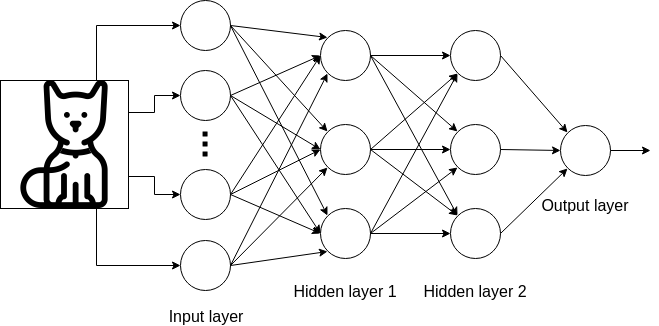
\includegraphics[width=\textwidth]{./pictures/method/example_neural_network.png}
    \caption{Example neural network that illustrates how neurons are organized
        into different layers with a special input layer and a special output
        layer. The neurons in the input layer are connected to individual pixels
        in an input image and the output layer is a single neuron computing the
        probability that the image contains a cat.}
    \label{fig:example_nn}
\end{figure}

There are different kinds of layers. The layers depicted in Figure
\ref{fig:example_nn} are Dense layers.

\begin{description}
    \item[Dense Layer:] TODO
    \item[Convolutional Layer:] TODO
    \item[\gls{LSTM} Layer:] TODO
    \item[\gls{GRU} Layer:] TODO
    \item[Embedding:] TODO
\end{description}

\subsubsection{TODO: Backpropagation}\label{sec:BP}

The neural network learns by updating the weights in the network. The weights
are updated using \gls{BP}. The process can be split into three distinct steps
which are continuously repeated:

\begin{enumerate}
    \item Feed Forward,
    \item Back Propagate,
    \item Update Weights.
\end{enumerate}

The goal of these three steps is to minimize the overall cost of the network.
The cost in this case, refers to the loss we end up with. In order to do so,
all we have to to do i step in the direction of the negative gradient as this
points to where the minimum cost can be found. In order to do so however, we
have to know the gradient of the cost function, in other words we need to find
the derivative. For us to do this, we have consider the cost function and the
network for what it is, a series of functions taking as an argument the result
of a previous function, and a weight, as per the equation \ref{eq:neuron}. This
process from goes back all the way from the cost function to the initial input.
As such, we have to make use of the chain rule in order to have a chance of
computing the gradient of out loss function.

\begin{definition}[Chain Rule]
    
    If functions \textbf{f} and \textbf{g} er both differentiable and
    \textbf{F} is the composite function defined by $F(x) = f(g(x))$,
    where $F' = f'(g(x)) \cdot g(x)$,

\end{definition}

In order to that the network makes use of the gradient to optimize each of
the individual weights. Step 1, feeding forward, is simply a pass through the
\gls{NN}. When this is done with singular training sample, we end up with a
final cost of the network for that single training sample. It is this cost that
back propagation attempts to optimize on. On order to do so all one simply
has to do is step in direction of the negative gradient of the cost function.
The cost function however is of cause dependent on outputting layer. Each
neurons at these layers have 3 values we can choose to optimize our gradient
on. The bias, the wight, and our choice of activation function. In the case of
back propagation, it is with respect to the weights, we want to optimize our
cost function. Using the gradient with respect to the weights of each neuron
contributing the cost function, we can compute a set of desired changes to
those desired that seek to optimize the output of the neuron. This is done
for all neuron in the layer, ending up with a set of desired weight changes
for each neuron in the layer. All the changes a summarized and then applied
to that former layer, enabling that same process to be performed recursively
back through the network, which is Step 2. Back Propagate. This is done for all
the training samples in our training set, ending up with each training sample
having a set desired weights. All these desires are then average, and applied
to the network, which is Step 3. Update Weights. That final averaged set of
weight are essentially the negative gradient of the cost function, which we
step in the direction of using. A step of a size, specified by the learning
rate. This process of back propagation however, is really computationally heavy
as each training sample has to be processed. As such, in practice the training
data is shuffled, and split into batches which are then fed to the network.
This means that the final result of the back propagation wont be the actual
negative gradient of the cost function, but rather a very close approximation,
a difference which is negligible after repeated runs of the back propagation
algorithm.

In order to explain this using a more mathematical approach, we need to chose
a activation function as our example, as it is with regard to that we find our
gradient. In this case we chose the sigmoid activation function, as it was
the more easy one to work with.

$$
\sigma(x) = \frac{1}{1 + e^{-x}}
$$

The derivative of which is of cause:

\begin{align}
\frac{d}{dx}\sigma(x) &= \frac{d}{dx}(\frac{1}{1 + e^{-x}})\\
&= \frac{e^{-x}}{(1+e^{-x})^2}
\end{align}

TODO: More math!


\subsubsection{Activation Functions}
The activation function $h$, used at each neuron, defines the output of the
node given a certain input. A simple example of this would be computer chip
circuit, which can be seen as a series of activation functions outputting 0 or
1 depending on their input. This activation function would be a linear one.
When applying activation functions to neurons in \gls{NN}s, they are usually
non-linear, as it allows for the computation of more complex problems using a
smaller amount of neurons, relative to usage of a linear activation function,
as they allow for the universal function approximation, a point also made by
\cite{6797088}

A plot of different activation functions is shown in Figure
\ref{fig:activation_functions}.

\begin{figure}
    \centering
    \textbf{Activation Functions}\par\medskip
    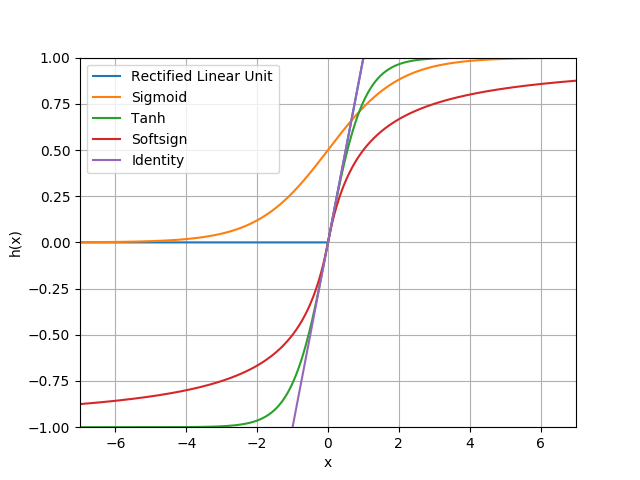
\includegraphics[width=0.5\textwidth]{./pictures/method/activation_functions.png}
    \caption{Different activation functions that can be used in neural
        networks.}
    \label{fig:activation_functions}
\end{figure}

Each activation function has its pros and cons. We mainly made use of the
\gls{ReLu} activation function in the hidden layers of our networks. The
reason for this selection is its general purpose use. When selecting an
activation function for your neurons, the best function would be the one which
best approximates the underlying function. Without a good idea as to what
that function might be, \gls{ReLu} is a good starting point. Its simplicity
provides a quick computation time, and its below zero limitation means that a
large portion of the network won't be activating, resulting in an even smaller
computation time. In addition to that, the derivative of the function is 1
in the case of a positive input, resulting in the \gls{BP} loss having equal
influence throughout the network. In the case of other activation functions,
this might not be the case, resulting in an altering of the error as we
propagate backwards through the network. This could lead to a big error in the
deeper layers not reaching the shallow layers of the network. This property of
the \gls{ReLu} activation function, does however not come without its costs.
If the learning rate of the network isn't configured correctly, a \gls{ReLu}
activated neuron might be blasted with a gradient so large, that it never
reaches a point of activation again. In other words, the neuron "dies". As
such, one can risk a network containing a lot of dead non-activation neurons,
thus greatly decreasing its quality. On the other hand the sigmoid function,
doesn't allow its neurons to die. It can become victim to saturation. In
the case of weight being too small or too high, the output values will be
placed at the far ends of the sigmoid range of values. At this point the
gradient is incredibly small, meaning that the contribution that neuron now has
is negligible. This neuron is now only a strain on the network, slowing it
down through its activation, but contribution nothing, a problem \gls{ReLu}
does not have. Its based on these considerations we chose the \gls{ReLu}
activation function, leaving us the task of properly selecting our learning
rate.\cite{JiYan, AndrejKarpathy, AvinashSharmaV}

As the activation function of our output neurons we have generally
used the softmax function. The softmax function is shown in Figure
\ref{fig:softmax_activation}. The function is defined as

\begin{equation}
    h(x_i) = \frac{e^{x_i}}{\sum_{k=1}^n e^{x_k}}, \text{for $i = 1 \dots n$}.
\end{equation}

The softmax function takes any vector $x \in \mathbb{R}^n$ and returns a vector
$y \in (0, 1)^n$. Where the sum of the output vectors elements will be equal to
1. The function is therefore great at constructing a probability distribution
based on an input vector. Each individual value in the vector get a high
probability if the value is high and a low probability if the value is low.
Therefore the function is often used at the end of networks to get the
probability of each class in a classification problem.

\begin{figure}
    \centering
    \textbf{Softmax Activation Function}\par\medskip
    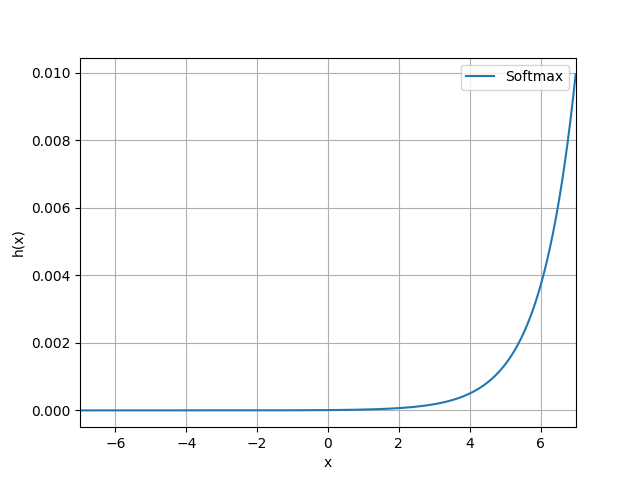
\includegraphics[width=0.5\textwidth]{./pictures/method/softmax_function.png}
    \caption{The softmax activation function.}
    \label{fig:softmax_activation}
\end{figure}

\subsubsection{Siamese Networks}

Classical machine learning approaches for text analysis and all our baseline
methods are based on handcrafted feature sets. Deep learning has shown
promising results in extracting features from raw images and raw text
\cite{hongxiaosunyuan}. We wanted to use deep learning to automatically learn
features from a large amount of data. At the same time we want to solve the
MaCom problem. Siamese neural networks are as described earlier networks that
compares two inputs. The networks has been used by \cite{Koch2015SiameseNN},
\cite{NIPS1993_769} and \cite{qian:2018} for comparing text, images and
signatures. \cite{qian:2018} use a Siamese network but with no convolutions and
a distance function on top for text analysis while \cite{Koch2015SiameseNN}
used a Siamese network with convolutions and fully connected network on top for
image analysis. Our approach is to use convolutions in the Siamese network to
learn important features from the texts. We also use a fully connected network
on top of the convolutional layers to learn from the features the convolution
extracted. An example of this architecture can be seen in Figure
\ref{fig:siamese_example}.

\begin{figure}
    \centering
    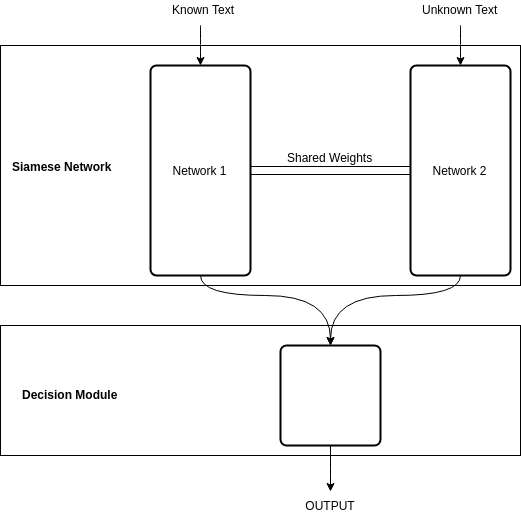
\includegraphics[scale=0.5]{./pictures/method/Siamese.png}
    \caption{The basic architecture of a Siamese neural network, which takes in
        two sources of data, and runs it through two parallelle networks,
        sharing their weights at each layer}
    \label{fig:siamese_example}
\end{figure}

The network will take two inputs, a text $t_k \in T_\alpha$ and a text $t_u
\in T_\beta$. The network will then try to figure out whether $\alpha =
\beta$. The convolutions in the network will look at $n$ characters at a
time and give an output. Therefore the convolutional layers will be able to
learn important n-grams and extract a representation of $t_k$ and $t_u$. This
representation will be given to some dense layers which will learn how to
compare the feature-sets extracted. The Siamese part of the network is the
convolutional part of the network which will share weights when extracting
n-grams from the two texts.

The final output of the network will be a probability that $\alpha = \beta$.
Since the MaCom dataset consist of multiple known texts per author and this
network architecture only compares two texts we define a separate system for
making the final prediction.

\subsection{Prediction System}

In the MaCom problem we are given a set of texts for each author so we can make
use of multiple texts when making our predictions. We can also use metadata
about the individual texts to make our prediction. An advantage of using
multiple texts for each author to make a prediction is that outliers will be
averaged out.

\begin{definition}[Prediction System]

    \label{def:prediction_system}

    Our prediction system is a function $P(f, w, \alpha, t_{unkown}, \theta)
    \in \{0, 1\}$ where $f$ is a function taking two texts and giving the
    probability that the texts are written by the same author, $\alpha$ is an
    author, $t_{unknown}$ is a text of unknown authorship, $w$ is a function
    $w:T_\alpha \rightarrow [0,1]$ where $\sum_{t_{known} \in T_\alpha}
    w(t_{known}) = 1$ and $\theta \in [0,1]$. The prediction system then
    returns,

    \begin{equation}
        P(f, w, \alpha, t_{unkown}, \theta) = \begin{cases}
            1 & \text{if } \sum_{t_{known} \in T_\alpha} w(t_{known}) f(t_{known}, t_{unkown}) > \theta \\
            0 & \text{otherwise}.
        \end{cases}
    \end{equation}

\end{definition}

That is the prediction system returns 1 if the weighted average of the
probability that $t_{unknown}$ is written by the same author as $t_{known}$ for
each $t_k \in T_\alpha$ is greater than the threshold $\theta$ and 0 otherwise.

The $f$ parameter can be anything that takes two texts and returns a
probability. We are going to present several different networks that can be used
as $f$ as they will take two texts and end with a softmax layer that outputs a
probability distribution.

The $w$ parameter in the prediction system can be used to weigh the known
texts differently. The most obvious weighing scheme is to just use a uniform
weighting. That way we simply take an average of the predictions of our networks
over the different texts an author has written. We define all the following
weight functions as functions taking a sequence of texts written by the same
author in chronological order and returning a sequence of weights in the same
order. The weight function were used in \ref{def:prediction_system} as a
function of a single text $t$ and in that use case it simply returns the weight
given to that particular text in the following definitions.

\begin{definition}[Uniform Weighing]

    The uniform weight function $w_\mathcal{U}(T) \in [0.0, 1.0]$
    where $T$ is a sequence of texts written by the same author $\alpha$ in
    chronological order, computes the weights as,

    \begin{equation}
        w_\mathcal{U}(T_1), w_\mathcal{U}(T_2), \dots, w_\mathcal{U}(T_n) =
        \frac{1}{n}, \dots, \frac{1}{n}
    \end{equation}

\end{definition}

The uniform weight function does not use any information we have about the
texts. It is mostly part of our weight functions as a sort of baseline to
make sure we don't make any weight functions that are worse than a simple
uniform weighing. Our other weight functions makes use of metadata we know
about the texts. As an example we have a timestamp of when a text was turned
in to the MaCom servers. We therefore know when the text was written and
we assume that newer texts will better reflect the current writing style
of a studen than older texts. We have therefore defined several weight
functions using the times the texts was written. In the following we let
$\tau$ be a function that returns the number of seconds since the epoch
\footnote{https://en.wikipedia.org/wiki/Unix\_time} that the text was turned in
at. We start with a simple weight function where the newest text has weight
$\frac{1}{2}$, the second weight $\frac{1}{4}$ and so on.

\begin{definition}[Time Weighted Simple]

    The time weighted simple function $w_s(T) \in [0.0, 1.0]$ where $T$ is a
    sequence of texts written by the same author $\alpha$ in chronological
    order, computes the weights as,

    \begin{equation}
        w_s(T_1), w_s(T_2), \dots, w_s(T_n) = \frac{1}{2^1}, \frac{1}{2^2},
        \dots, \frac{1}{2^{n-1}}, \frac{1}{2^{n-1}}
    \end{equation}

\end{definition}

The problem with the simple time weighted function is that it only looks at the
order in which the texts are written and not the actual times they were written
at. It is clear that the newest text should not be weighed twice as important as
the second newest if they are only turned in a single day apart. We therefore
defined a function that also took into account the relative time between the
texts.

\begin{definition}[Time Weighted Relative]

    The relative time weighted function $w_r(T) \in [0.0, 1.0]$ where $T$ is a
    sequence of texts written by the same author $\alpha$ in chronological
    order, computes the weights as,

    \begin{equation}
        w_r(T_1), w_r(T_2), \dots, w_r(T_n) =
            \frac{\tau(T_1) - \min_{t \in T} \tau(t)}{\sum_{t \in T} \tau(t)},
            \frac{\tau(T_2) - \min_{t \in T} \tau(t)}{\sum_{t \in T} \tau(t)},
            \dots,
            \frac{\tau(T_n) - \min_{t \in T} \tau(t)}{\sum_{t \in T} \tau(t)},
    \end{equation}

\end{definition}

There the first text will get the lowest weight since $T_1$ is smaller than
$T_2$ and the time between individual texts are taken into account. The problem
with that definition is mainly that the first text $T_1$ will always have weight
0 since $\min_{t \in T} \tau(t) = T_1$. We are guessing that even the oldest
text we have available will provide some information to the prediction system.
Another problem is that texts written even a few days apart are rated very
different since we use the number of seconds since the epoch as the timestamps.
We therefore defined yet another weighing function that still takes into account
the time between texts but considers texts written in the same month to have the
same timestamp. Furthermore it arbitrarily adds one to all the times to prevent
the first text to get weight 0. In the following the function $\tau_m$ returns
the number of months since the epoch a text was written.

\begin{definition}[Time Weighted Relative Monthly]

    The relative time weighted function $w_{rm}(T) \in [0.0, 1.0]$ where $T$ is
    a sequence of texts written by the same author $\alpha$ in chronological
    order, computes the weights as,

    \begin{align}
        w_{rm}(T_1), w_{rm}(T_2), \dots, w_{rm}(T_n) =&
            \frac{(\tau_m(T_1) - \min_{t \in T} \tau_m(t)) + 1}{\sum_{t \in T} \tau_m(t)},
            \frac{(\tau_m(T_2) - \min_{t \in T} \tau_m(t)) + 1}{\sum_{t \in T} \tau_m(t)}, \\
            & \dots,
            \frac{(\tau_m(T_n) - \min_{t \in T} \tau_m(t)) + 1}{\sum_{t \in T} \tau_m(t)}
    \end{align}

\end{definition}

TODO: Define a weight function that also looks at the length of the texts.

To get an idea of the weights the different functions produce we made a bar
plot using the texts of a random student in our dataset shown in Figure
\ref{fig:weights_bar}. The first text in the plot is the oldest and the last is
the newest.

\begin{figure}
    \centering
    \textbf{Example application of weight functions}\par\medskip
    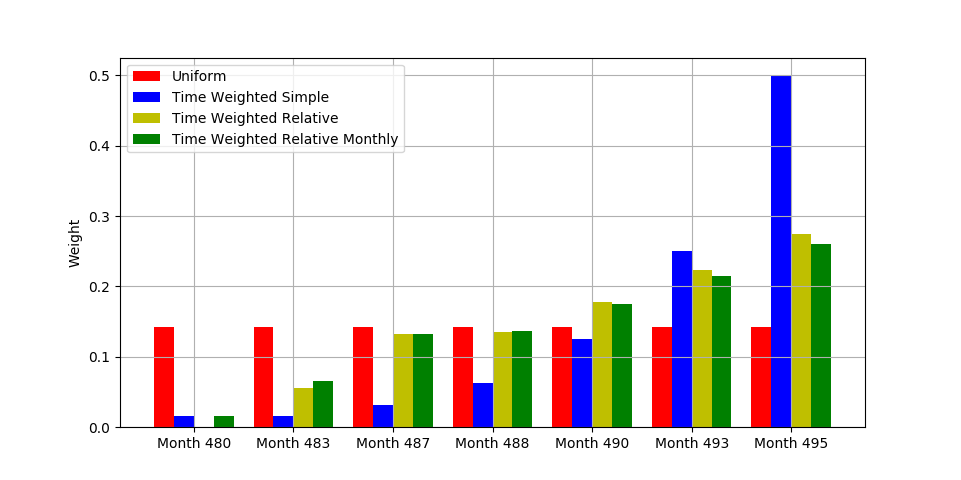
\includegraphics[width=\textwidth]{./pictures/method/weight_bar.png}
    \caption{The weights given to texts with different timestamps using
        different weight functions.}
    \label{fig:weights_bar}
\end{figure}

The $\theta$ parameter in the prediction system determines when we consider an
unknown text to be written by an author. The natural choice for $\theta$ is 0.5
since that is what the network use when it computes the loss of each training
sample. However the $\theta$ parameter can be used to enforce how sure we have
to be of a decision to accuse an author of not having written an assignment. As
described earlier MaCom does not want to accuse innocent students of cheating.
That means that it is very important to MaCom to minimize the number accusation
error. We can use the $\theta$ parameter to control that error. Hopefully the
\gls{FN}s generally end up with a value closer to 1 than the \gls{TN}s. If that
is the case then lowering $\theta$ value will lower the fraction since there
will be fewer \gls{FN}s. That might lower the overall accuracy of the prediction
system but will make sure that at few students as possible are falsely accused.
